% # 公立はこだて未来大学・修士論文テンプレートファイル(unicode)
%
% ## 改訂履歴:
% - 2019/12/01 初版 作成者:三上貞芳
% - 2020/01/12 V1.2 作成者:三上貞芳 英字綴訂正
%
% ## 論文作成の手順
%
% 1. 以下のtexファイルを作成してください
% - cover.tex           氏名・タイトル等の表紙情報
% - eabstract.tex       英語アブストラクト
% - jabstract.tex       日本語アブストラクト
% - chapterX.tex        本文第X章
% - publications.tex    発表・採録等の実績(確定分も含む)
% - acknowledgment.tex  謝辞
% - bibliography    .tex    参考文献
%
% 2. このテンプレートの「TODO: 本文」以下に,作成した章に対応する\input{chapterX.tex}文を追記してください(Xは章番号)
%
% 3. このテンプレートとfunstyle_master.texと合わせてuplatex環境でコンパイルし,PDFを作成します.
%

\documentclass[uplatex, a4paper, report, 11pt, oneside]{jsbook}

% packages
\usepackage[utf8]{inputenc}
\usepackage[dvipdfmx]{graphicx}
\usepackage{lmodern}             % use latin modern font
\usepackage{amsmath,amssymb,amsthm}

\usepackage{layout}
\usepackage{enumerate, multirow}

% 未来大書式設定
% % # 公立はこだて未来大学・修士論文書式定義ファイル
%
% (https://github.com/kmiya/naist-thesis-tmpl を一部参照)
% 
% ## 改訂履歴:
% - 2019/11/18 初版 作成者:三上貞芳

% ## 使用法;
% - main.texを参照してください.
% - **このファイルを変更する必要はありません**

\usepackage[dvipdfmx]{graphicx}
\usepackage[utf8]{inputenc}
\usepackage[T1]{fontenc}
\usepackage{lmodern}
\usepackage{amsmath,amssymb,amsthm}
\let\equation\gather
\let\endequation\endgather
\usepackage{fancybox}
\usepackage[flushmargin,symbol]{footmisc}
\usepackage[nottoc]{tocbibind}
\usepackage[dvipdfmx,%
 bookmarks=true,%
 bookmarksnumbered=true,%
 setpagesize=false,%
 colorlinks=false,%
 linkbordercolor={0.8 0.8 0.8},%
 citebordercolor={0.8 0.8 0.8},%
 pdfborder={0 0 0.6},%
% urlcolor=black,linkcolor=black,citecolor=black,%
 pdftitle={},% 修論のタイトルを入れる
 pdfauthor={},% 名前を入れる
 pdfsubject={Master's thesis},%
 pdfkeywords={\ekeywords}]{hyperref}
\usepackage{pxjahyper}

% ページレイアウト
\textheight=20.6truecm          % 縦
\textwidth=14.5truecm           % 横
\oddsidemargin=0.6truecm        % 左マージン(1inオフセット後)
\evensidemargin=-3.8truecm      % 右マージン(1inオフセット後)

% フォント等調整
% 参考文献
\def\thebibliography#1{\chapter*{参考文献\markboth
 {参 考 文 献}{参 考 文 献}\addcontentsline{toc}{chapter}{参考文献}}\list
 {[\arabic{enumi}]}{\settowidth\labelwidth{[#1]}\leftmargin\labelwidth
 \advance\leftmargin\labelsep
 \usecounter{enumi}}
 \def\newblock{\hskip .11trueem plus .33trueem minus -.07trueem}
 \sloppy
 \sfcode`\.=1000\relax}
\let\endthebibliography=\endlist

% 章
\makeatletter%%
\def\@makechapterhead#1{\hbox{}%
  \vskip-1\Cvs
  {\parindent\z@
%  \reset@font\LARGE\bfseries
   \raggedright\reset@font\Large\bfseries% 左揃え
   \ifnum \c@secnumdepth >\m@ne
     \setlength\@tempdima{\linewidth}%
     \vtop{\hsize\@tempdima%
         \@chapapp\thechapter\@chappos\mbox{\ \ }%
     #1}%
   \else
     #1\relax
   \fi}\nobreak\vskip1\Cvs}
\makeatother%%

\makeatletter%%
\def\@makeschapterhead#1{\hbox{}%
  \vskip-1\Cvs
  {\parindent \z@ \raggedright
    \normalfont
    \interlinepenalty\@M
    \Large\headfont #1\par\nobreak
    \vskip1\Cvs}}
\makeatother%%

% 節
\makeatletter%%
\renewcommand{\section}{%
  \@startsection{section}% #1 見出し
   {1}% #2 見出しのレベル
   {\z@}% #3 横組みの場合,見出し左の空き(インデント量)
   {1.5\Cvs \@plus.5\Cdp \@minus.2\Cdp}% #4 見出し上の空き
   {.5\Cvs \@plus.3\Cdp}% #5 見出し下の空き (負の値なら見出し後の空き)
  {\raggedright\reset@font\large\bfseries}% 左揃え
}%
\makeatother%%

% 小節
\makeatletter%%
\renewcommand{\subsection}{%
  \@startsection{subsection}% #1 見出し
   {1}% #2 見出しのレベル
   {\z@}% #3 横組みの場合,見出し左の空き(インデント量)
   {1.5\Cvs \@plus.5\Cdp \@minus.2\Cdp}% #4 見出し上の空き
   {.5\Cvs \@plus.3\Cdp}% #5 見出し下の空き (負の値なら見出し後の空き)
  {\raggedright\reset@font\normalsize\bfseries}% 左揃え
}%
\makeatother%%

% 表題
\makeatletter
\def\@startsection#1#2#3#4#5#6{%
  \if@noskipsec \leavevmode \fi
  \par
  \@tempskipa #4\relax
  \if@english \@afterindentfalse \else \@afterindenttrue \fi
  \ifdim \@tempskipa <\z@
    \@tempskipa -\@tempskipa \@afterindentfalse
  \fi
  \if@nobreak
    \everypar{}%
  \else
    \addpenalty\@secpenalty
    \ifdim \@tempskipa >\z@
      \vskip\@tempskipa
      \if@slide\else
        \null
        \vspace{-\baselineskip}%
      \fi
    \fi
  \fi
  \noindent
  \@ifstar
    {\@ssect{#3}{#4}{#5}{#6}}%
    {\@dblarg{\@sect{#1}{#2}{#3}{#4}{#5}{#6}}}}
\makeatother

% 式番号
\makeatletter
  \renewcommand{\theequation}{%
  \thesection.\arabic{equation}}
    \@addtoreset{equation}{section}
\makeatother


% 図番号
\makeatletter
 \renewcommand{\thefigure}{%
  \thechapter.\arabic{figure}}
   \@addtoreset{figure}{chapter}
 \makeatother
\makeatletter

% 目次に小節を表示
\setcounter{tocdepth}{4}


% TODO: タイトル・著者等の情報
% TODO: 論文題目等の情報を以下に記入

\newcommand{\jdoctitle}{修士論文}
\newcommand{\edoctitle}{Master's Thesis}
\newcommand{\jtitle}{雰囲気推定を用いた\\作業通話マッチング支援サービスの提案}  % 修論の題名
\newcommand{\etitle}{Proposal of a Work Call Matching Support System\\Using Atmosphere Estimation}   % 論文題目(英)
\newcommand{\jauthor}{立花 虎太郎}      % 著者名(日)
\newcommand{\eauthor}{Tachibana Kotraro} % 著者名(英)
\newcommand{\jadvisor}{奥野 拓}   % 指導教員名(日)
\newcommand{\eadvisor}{Okuno Taku}  % 指導教員名(英)
\newcommand{\jdate}{2023年1月12日}  % 論文提出日   (日)
\newcommand{\edate}{January 12, 2023}  % 論文提出年月 (英)
\newcommand{\jkeywords}{作業通話, 対話雰囲気推定, コミュニケーション支援} % キーワード(日)
\newcommand{\ekeywords}{Work Call, Dialogue Atmosphere Estimation, Communication Support}   % キーワード(英)
\newcommand{\eshorttitle}{Work Call Matching Support System Using Atmosphere Estimation}    % 短縮英題題名(おおよそ8 words以内)
\newcommand{\jaffiliation}{高度ICT領域}    % 領域名(日)
\newcommand{\eaffiliation}{Advanced ICT Field}    % 領域名(英)


% TODO: 英語アブストラクト
% TODO: 英文アブストラクトを以下の{}内に記述(以下はダミーテキスト)
\newcommand{\eabstract}{

In recent years, "work calls”, in which multiple people work on individual tasks while sharing time via a call tool, have become widely used.
The purpose of this study is to support casual matching between users who have the same working preference but have weak relationship with each other in a work call inviting participants on SNS.
This study proposes a visualization method of how to proceed with a work call focusing on the dialogue atmosphere and a participant recruitment system using the visualization method.
This study uses machine learning to estimate the dialogue atmosphere.
The model is constructed using speech state temporal features that can provide highly accurate estimation of dialogue atmosphere while ensuring the privacy of participants.
This study constructs and verifies a model for estimating the atmosphere of a working conversation held with 2 to 4 speakers.

}

% TODO: 日本語アブストラクト
% TODO: 日本語アブストラクトを以下の{}内に記述(以下はダミーテキスト)
\newcommand{\jabstract}{

近年,複数人が通話ツールを介して時間を共有しながら,各々の個人作業に取り組む活動である「作業通話」が広く行われている.
本研究では,SNSを利用し参加者を募る作業通話の募集者に対して,作業の進め方の好みは一致しているが関係は希薄なユーザとの気軽なマッチングの支援を行う.
そのために対話雰囲気推定を用いた作業通話の進め方の可視化手法と,それを用いた参加者募集システムの提案を行う.
本研究では機械学習を用いた対話雰囲気推定を行う.
モデルの構築には,参加者のプライバシーを担保しながら高精度の対話雰囲気推定を行える発話状態時間特徴を用いる.
話者数2 〜 4名で開催される作業通話の対話雰囲気を推定するモデルの構築及び検証を行なった.

}


% page size
\textheight     = 22.6truecm
\textwidth      = 14.7truecm
\oddsidemargin  = 0.6truecm

% header and footer
\usepackage{fancyhdr}
\pagestyle{fancy}
\setlength{\footskip}{16pt}
\fancyhf{}
\renewcommand{\chaptermark}[1]{\markboth{\thechapter.\ #1}{}}
\rhead{\leftmark}
\renewcommand{\headrulewidth}{0pt}
\cfoot{\thepage}
\lfoot{~~ \\Master's thesis, Future University Hakodate}
\lhead{\eshorttitle}

%-------------------------------------
\begin{document}

\thispagestyle{empty}
\vspace*{1.5truemm}
\begin{center}
    \LARGE\bfseries
    修士論文
\end{center}
\vspace*{2truemm}
\begin{center}
    \LARGE\bfseries\jtitle
\end{center}
\vspace*{2em}
\begin{center}
    \large\bfseries 公立はこだて未来大学大学院~~システム情報科学研究科\par%
    \jaffiliation
\end{center}
\vspace*{1em}
\begin{center}
    \Large\bfseries\jauthor
\end{center}
\vspace*{1em}
\begin{center}
    \large 指導教員~~~~\jadvisor\par
    \vspace{0.5em}
    \large 提出日~~~~\jdate
\end{center}
\vspace*{3em}
\begin{center}
\textbf{\Large Master's Thesis}\par
\vspace*{2em}
\textbf{\Large \etitle}\par
\vspace*{1em}
{\normalsize by}\par
\vspace*{1em}
{\large \eauthor}\par
\vspace*{1.5em}
Graduate School of Systems Information Science, Future University Hakodate \par
\eaffiliation

% \vspace*{0.5em}
\normalsize Supervisor: \quad \eadvisor \par
\vspace*{2em}
Submitted on \edate
\end{center}
%\vspace*{\fill}

% 英語アブストラクト作成
\newpage
\thispagestyle{empty}
\vspace*{30truemm}
\noindent
\textbf{Abstract--}~
\eabstract

\vspace*{1em}
\noindent
\textbf{Keywords:}~ 
\ekeywords

% 日本語アブストラクト作成
\newpage
\thispagestyle{empty}
\vspace*{30truemm}
\noindent
\textgt{概~要:}~
\jabstract

\vspace*{1em}
\noindent
\textgt{キーワード:}~ 
\jkeywords


% 目次
\tableofcontents
\thispagestyle{empty}

% ページ番号初期化
\setcounter{page}{0}

% TODO: 本文
\chapter{序論\label{sec:introduction}}
\thispagestyle{plain}

\section{背景}

近年,「作業通話」と呼ばれる活動が広く行われている.
作業通話とは,複数人がDiscord\cite{Discord}等の通話ツールを介して時間を共有しながら,各々の個人作業に取り組む活動を指す.
作業通話にはいくつかの別称があり,コーディングを行うエンジニアの間では「オンラインもくもく会」,イラスト制作や小説の執筆を行うクリエイターや,勉強に取り組む学生の間では「さぎょいぷ」としても浸透している.

作業通話の開催には大きく二つの利点がある.
一つ目の利点として作業効率の向上が挙げられる.
作業通話は他者と通話をしながら作業を行うことから,常に他者の存在を感じながら作業を進めることができるという特性を持つ.
それにより,個人の経験や性格によって個人差があるものの,適度に他者の存在を感じることで観衆効果が発生し,作業効率が向上することが報告されている\cite{Zajonc}\cite{Matsumoto}\cite{Miyamoto}.
また,参加者同士で会話を行うことでリフレッシュ効果が期待できるほか,作業内容が類似している場合は作業中に生まれた疑問を即座に他の参加者に聞くことができるなど作業効率の向上が見込める点が多くある.
二つ目の利点として他者との関係構築の機会の増加が挙げられる.
特に参加者間の親密度の向上や新しいコミュニティの発見の機会につながる.
作業通話の参加者は常に他者と通話回線がつながっており,声を発するだけで会話が始められる状態である.
また,参加者には作業を進めるという目的があることから数十分から数時間に及ぶ作業時間になることが多い.
これらの特性から自然に会話が発生し,お互いの理解が深まる.
また,並行して作業も行なっていることから無理に会話を続ける必要もなく,心理的な負担も小さい.
加えて,SNS上で知り合った関係が希薄もしくは皆無な人(以下,「無縁ユーザ」)と作業通話を開催する文化も生まれ,作業通話はコミュニケーション媒体の一種として機能している.

一方で,作業通話の参加者には各々進め方の好み(以下,「作業嗜好」)があり,それが一致する参加者を募ることが難しいという問題がある.
作業通話には開催検索する時間帯,作業の類似性,利用するコミュニケーションツールなどの要素があり,参加者には会話量,性格などの要素がある.
作業嗜好が合わない参加者と長時間の作業通話は,前述した作業通話の利点を十分に活かすことができない場合がある.
作業通話の参加者を募る方法は大きく二つある.
一つは友人など既に所属しているコミュニティで参加者を募る方法(以下,「コミュニティ募集」)である.
コミュニティ募集は,身近な人を気軽に招待,依頼できる反面,募集対象者数が少ないため各々の都合や作業嗜好の違いによって十分に参加者が集まらない場合がある.
もう一つの募集方法として,Twitter\cite{Twitter}等のSNSを通じて不特定多数の人を対象として参加者を募る方法(以下,「SNS募集」)がある.
SNS募集は募集対象者数が多いため,その中に作業嗜好の合う人が存在する可能性が高い一方で,実際に利用されることは少ない.
これには大きく二つの要因がある.
一つ目は募集対象者が数ある募集の中からどれが自身の作業嗜好と合うものか判断することが困難であるという点である.
二つ目に募集者が無縁ユーザに対して参加者を募ることや,募集対象者が募集に対して参加意思を表明することの心理的負担が大きいという点がある.
事実,Twitter上には「作業通話したいけど勇気がでない」といった投稿が多く見られる(図\ref{fig:search_results}).

\begin{figure}
    \centering
    \fbox{
        
\includegraphics[width=0.7\textwidth]{figs/search_results.jpg}
    }
    \caption{Twitterで「作業通話 勇気」で検索した結果}
    \label{fig:search_results}
\end{figure}

本研究では,これら二つの要因を解消することで,作業嗜好の合う無縁ユーザとの気軽なマッチングを実現し,より効果的な作業通話の開催機会の増加を目指す.

\section{目的}

本研究の目的は,作業嗜好の合う無縁ユーザの気軽なマッチングを実現し,より効果的な作業通話の開催機会の増加を目指すことである.
そのために,作業通話の音声やメタデータから作業嗜好を推定し,可視化及び無縁ユーザのマッチングを行うシステムを提案する.
特に,本研究では対話雰囲気に着目し機械学習を用いた対話雰囲気の推定を行うことで作業嗜好の効果的な可視化を目指す.

\section{章構成}

本論文は全\ref{sec:conclusion}章で構成されている.
第\ref{sec:introduction}章では,本研究の背景と研究目的について述べた.
第\ref{sec:approach}章では,本研究のアプローチについて述べる.
第\ref{sec:related_researchs}章では,本研究に関連する研究について述べる.
第\ref{sec:proposal_system}章では,本研究で提案するシステムについて述べる.
第\ref{sec:estimation_model}章では,本研究で構築した対話雰囲気推定モデルについて述べる.
第\ref{sec:evaluation_experiment}章では,評価実験について述べる.
第\ref{sec:conclusion}章では,まとめと今後の展望について述べる.

\chapter{アプローチ\label{sec:approach}}
\thispagestyle{plain}

本章では第\ref{sec:introduction}章で述べた問題に対する本研究のアプローチについて述べる.
第\ref{sec:introduction}章では以下の問題について述べた.

\begin{enumerate}[i.]
    \item 自身と近い作業嗜好を持つ人の募集を探すことが困難
    \item 参加の意思表明の心理的負担が大きい
\end{enumerate}

\section{自身と近い作業嗜好を持つ人の募集を探すことが困難}\label{node:approach_i}

本問題の原因の一つに作業通話の募集文に作業嗜好を判断する情報が少ないことが挙げられる.
特に開催時間や募集人数,開催場所などの情報が欠落していることが多い(図\ref{fig:tweet_recruitment}).
コミュニティ募集の場合,募集対象者は募集者の人柄や作業の進め方などは事前に把握していることが多いためこの問題は無視されることが多い.
一方,SNS募集の場合,募集者の人柄から自身の作業嗜好との相性を推察することができないため募集対象者の参加意欲を減衰させている可能性が高い.

この問題の解決には作業嗜好の可視化が効果的であるといえる.
作業通話の募集概要(募集対象者や開催時間など)を募集文に明示することで,募集対象者は参加するかの判断に必要な情報の多くを把握できる.
しかし,作業嗜好の要素として雰囲気の好みが挙げられるが,これについては募集概要から推察することは困難である.
作業通話における雰囲気(対話雰囲気)は参加者の気構えや心情が深く関わっており,作業の進め方や参加者の満足感に強く影響を与える要素である.
したがって,本研究では対話雰囲気が作業嗜好の大きな要素になると仮定し,対話雰囲気を推定し可視化するシステムの構築を行う.
また,本研究では対話雰囲気を「盛り上がり」,「真面目さ」など複数人からなる対話における場の空気感と定義する.

\begin{figure}
    \centering
    \fbox{
        
\includegraphics[width=0.7\textwidth]{figs/tweet_recruitment.jpg}
    }
    \caption{Twitterで「作業通話 募集」で検索した結果}
    \label{fig:tweet_recruitment}
\end{figure}

\section{参加の意思表明の心理的負担が大きい}

本問題の原因として,無縁ユーザとの作業通話という文化が十分に浸透していないことが挙げられる.
加えて,募集は募集以外の投稿と混在しながらフランクに投稿されている場合も多い.
また,\ref{node:approach_i}節の問題も加わり募集文を見ただけではその募集がコミュニティ募集とSNS募集どちらなのかを判断することが難しいという問題もある.
これらのことから,募集対象者は興味のある募集を発見しても参加の意思表明をする心理的負担が大きいといえる.

そこで本研究では,\ref{node:approach_i}節で述べたアプローチに加え,参加の意思表明の心理的負担の軽減を目的にSNS募集の枠組みを提案する.
具体的には,SNS募集における募集文(ツイート)を生成できるシステムの提案を行う.
またこのシステムは,SNS募集対象者が自身に向けて募集が行われていることや,そのような募集方法が存在することを明確に認知することで参加の意思表明の心理的負担の軽減を目指している.
このシステムは,システムを通したコミュニケーションは受け入れやすいということが報告されていることからも一定の効果が期待できる\cite{Harada}\cite{Kimura}\cite{Nishimura}\cite{Tsuzuki}.
このシステムを用いて作成された募集文には,\ref{node:approach_i}節で述べた募集概要や対話雰囲気も併せて掲載することで,作業の透明性の向上を図りさらなる心理的負担の軽減を目指す.

\chapter{関連研究\label{sec:related_researchs}}
\thispagestyle{plain}

本研究では,遠隔で複数人によって行われる対話の雰囲気の推定と,その結果を用いたSNS上で行われるコミュニケーションの支援を目指している.
本章では,その上で本研究に関する研究について述べる.
はじめに,対話雰囲気推定を行っている研究について述べる.
次に,SNS上で行われるコミュニケーションを支援している研究について述べる.

\section{対話雰囲気推定に関する研究}
近年,人間と適切な会話を行う対話エージェントを開発するために,対話の雰囲気を推定する研究が数多く行われている.

人間同士の対話を対象とし,対話雰囲気推定を行った研究として徳久ら\cite{Tokuhisa}の研究がある.
徳久らは対話内容に対してDialogue Act (DA)とRhetorical Relation (RR)を用いた発話分類を行い,対話の盛り上がりとの関係を分析している.
DAとは,各対話内容が「質問」や「要求」,「提案」などのどのようなカテゴリに属するかをラベル付けする手法である.
DAが発話にラベル付けする手法に対し,RRは修辞構造を表す手法である.
結果として,言及される内容の主観性や,「嬉しい」や「つらい」などの感情に関する発話が盛り上がりとの関係が深いことが明らかになっている.
しかし,言語情報を実際の対話から抽出し,会話内容に基づいたラベル付けをし利用することは難しいことも示唆された.

仕草や表情等の非言語情報を用いた対話雰囲気の推定を行った研究として伊藤ら\cite{Ito}の研究がある.
伊藤らは,二者間の対話における盛り上がりに関与する要素を話者の動作や発話から分析している.
結果として,対話の盛り上がりを判断する要素として,発話の重なりやうなずき,笑い等の要素の重要度が高いことが明らかになっている.
また,頭部の動作特徴が場の雰囲気表現に有効であることが示唆された.
しかし,表情認識や動作認識は高いコストを必要とするため,リアルアイムの人間の会話に介入することは難しいという問題がある.
また,遠隔で行われる対話においても,これらの非言語情報が失われるため推定が困難である.

容易に抽出可能な特徴を用いて,対話の雰囲気を推定する研究として豊田ら\cite{Toyota}の研究がある.
豊田らは,発話時間特徴と主観評価を用いた機械学習によって対話雰囲気の推定を試みている.
対話の雰囲気を推定する学習済みモデル(以下,「対話雰囲気推定モデル」)はTree-Augmented Naive Bayes分類器(TAN)と遺伝的アルゴリズムを用いた特徴量選択が採用されている.
モデル構築の過程では,二者の発話全体における同時発話時間の占有率が比較的高い場合,対話が盛り上がっていると推定される傾向があることが明らかになっている.
また,対話をリードしている話者の発話の分散に対して,追従している話者の発話の分散が比較的高い場合にも,対話が盛り上がっていると推定されることが示されている.
構築した対話雰囲気推定モデルを5分割検証法によって分析した結果,「盛り上がり」,「真面目さ」,「親密さ」の推定において80\%を超える全体正答率が示されている.
豊田らの手法は,遠隔で行う対話の雰囲気推定も容易に行える反面,二者対話のみを想定しているため複数人での対話における対話雰囲気推定モデルの精度が確認されていない.
しかし,対話雰囲気推定モデルが高い水準で正しい雰囲気推定を行えていることから,豊田らのモデル構築手法を参考に本研究は対話雰囲気推定モデルを構築する.

\section{SNS上で行われるコミュニケーションに関する研究}

SNS上における繋がりの構築を支援する研究として北村ら\cite{Kitamura}や田村ら\cite{Tamura},久米ら\cite{Kume}の研究がある.
北村らは,関与ベースに基づくTwitterユーザの推薦を行い手法の有効性を示している.
田村らは,Twitterユーザにおける他者とのコミュニケーション量に基づいた会話しやすいユーザの推薦手法を提案している.
久米らは,コンテンツベースの推薦手法にカテゴリ情報を付加し,特徴語抽出手法であるTF-IDF法に各カテゴリへの興味度合いを示す「興味領域」という指標を加えたユーザ推薦手法を提案している.
これらの手法は,ユーザと相性の良い他のユーザを見つける上では有用だが,実際に繋がりを構築する上でユーザは推薦されたユーザに対して接触を図る必要があり,その際の心理的負担は考慮されていない.

SNS上での募集行為を支援する研究として樋川\cite{Hikawa}の研究がある.
樋川は,LINE \cite{LINE}上で実験協力者の募集を,Botを通して行うことができるシステムの構築・評価を行っている.
Botを用いることで適切な距離感の被験者候補に対して募集を行うことができたほか,希薄な関係の人同士におけるシステムを介したコミュニケーションの有効性が示唆された.

\chapter{提案システム\label{sec:proposal_system}}
\thispagestyle{plain}

本章では,本研究で提案するシステムについて述べる.

\section{概要}

本研究で提案するシステムの構成を図\ref{fig:matching_system_big_arrow}に示す.
本システムは,対話雰囲気推定モジュール(Discordのボイスチャンネルからデータベースまでのフロー)とそれを用いたマッチング支援モジュール(データベース以降のフロー)から構築される.
本システムでは開催された作業通話の音声をBotによって取得し,対話雰囲気を推定したのちに,その他のメタデータと共に記録しそれらを用いた支援を行う.
主なユースケースは作業記録の可視化と募集ツイートの生成の二つである.
作業記録の可視化では,それまでに集めたユーザ自身の活動嗜好や活動雰囲気のデータの統計値や傾向を算出し表示する.
募集ツイートの生成では,条件を入力することで可視化された自身のデータとともに新しく開催する作業通話の参加者を募るためのツイートを生成する.

\begin{figure}
    \centering
    \fbox{
        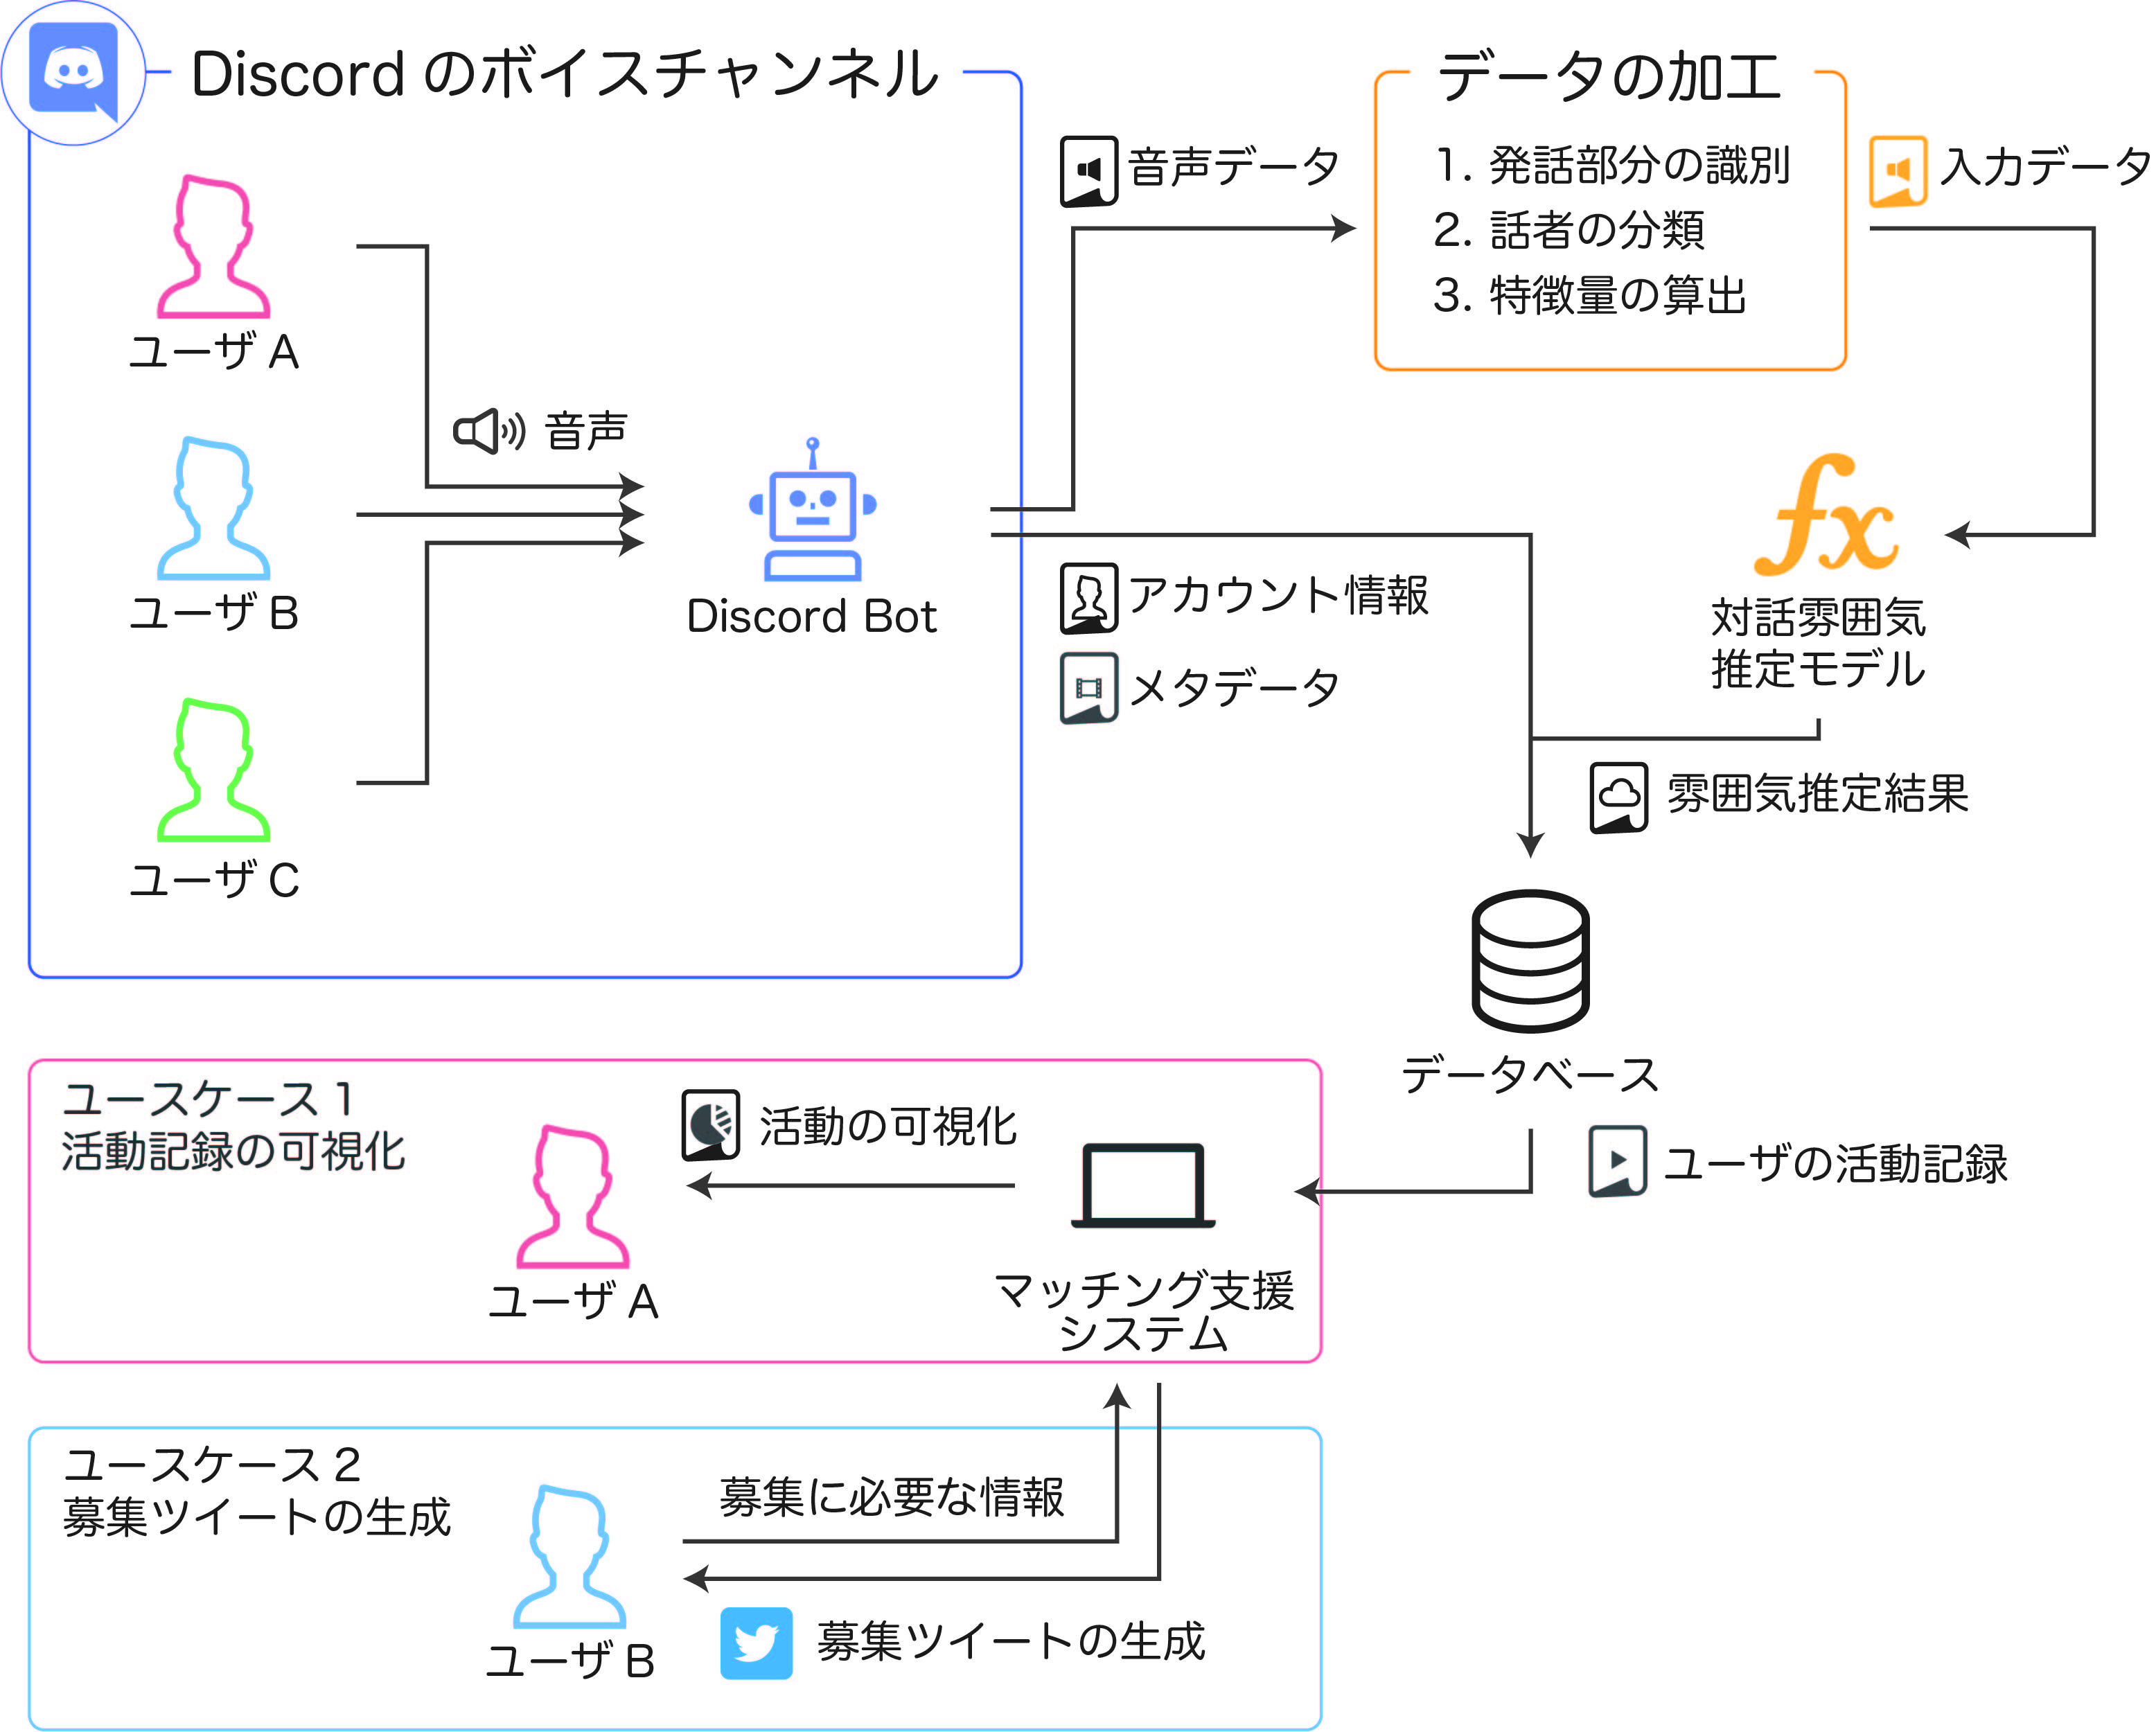
\includegraphics[width=0.7\textwidth]{figs/matching_system_big_arrow.jpg}
    }
    \caption{システムイメージ}
    \label{fig:matching_system_big_arrow}
\end{figure}

\section{対話雰囲気推定モジュール\label{node:estimation_module}}

本モジュールはDiscordで開催される作業通話を対象に,Botを作業通話に同席させBotを通して収集した情報から対話雰囲気を推定する.
対話雰囲気の推定には対話雰囲気に関する特徴量を学習した対話雰囲気推定モデルを用いる.対話雰囲気推定モデルの構築については第\ref{sec:estimation_model}章で詳細に述べる.

本モジュールでは,対話雰囲気推定のために音声データの収集を行う.
しかし,本研究で構築する対話雰囲気推定モデルでは言語情報を用いないため,誰がどのタイミングでどの程度発話したのかを基に算出した特徴量(以下,「発話時間特徴量」)のみを収集する.
これは第\ref{sec:related_researchs}章で述べた豊田らの手法を参考にしており,参加者のプライバシーに配慮しながらも高精度の推定を行えることから採用した.

Botの利用方法の想定を示す.
まず,Botはサーバに招待されることで利用可能状態となる.
作業通話を開始した際に開始用のコマンドをBotに対して入力することで録音を開始する.
作業通話が終了した際に終了用のコマンドを入力することで録音の停止と対話雰囲気の推定結果の出力をテキストチャンネル上に行う.
ユーザはそれを見て推定雰囲気の確認や主観的に正しいと感じた雰囲気への修正を行える.
それらのデータはサーバに記録される.記録したデータは再び学習データとしてモデルの精度向上に利用することを想定している.

\section{マッチング支援モジュール}

本モジュールは,3.1節のモジュールによって推定された対話雰囲気を用いてSNS募集及びその募集への参加の支援を行う.
本モジュールの対象はTwitterでのSNS募集である.
本モジュールは3.1節のモジュールより得た対話雰囲気推定結果と,募集を行うユーザの開催したい作業通話の概要の入力を行うことで募集用の投稿(図\ref{fig:tweet_image})を生成することを主機能としている.
本機能によって生成される投稿には,作業内容や開催時間帯,募集人数,これまでどのような雰囲気で活動する傾向があったかなどを掲載する.
また,次に示す作業嗜好の可視化機能によって可視化された作業嗜好も併せて掲載する.
本機能は,一目で無縁ユーザ向けの募集文であることがわかることと,開催したい作業通話の概要がわかることによって明確で効率的な募集形態を目指している.

\begin{figure}
    \centering
    \fbox{
        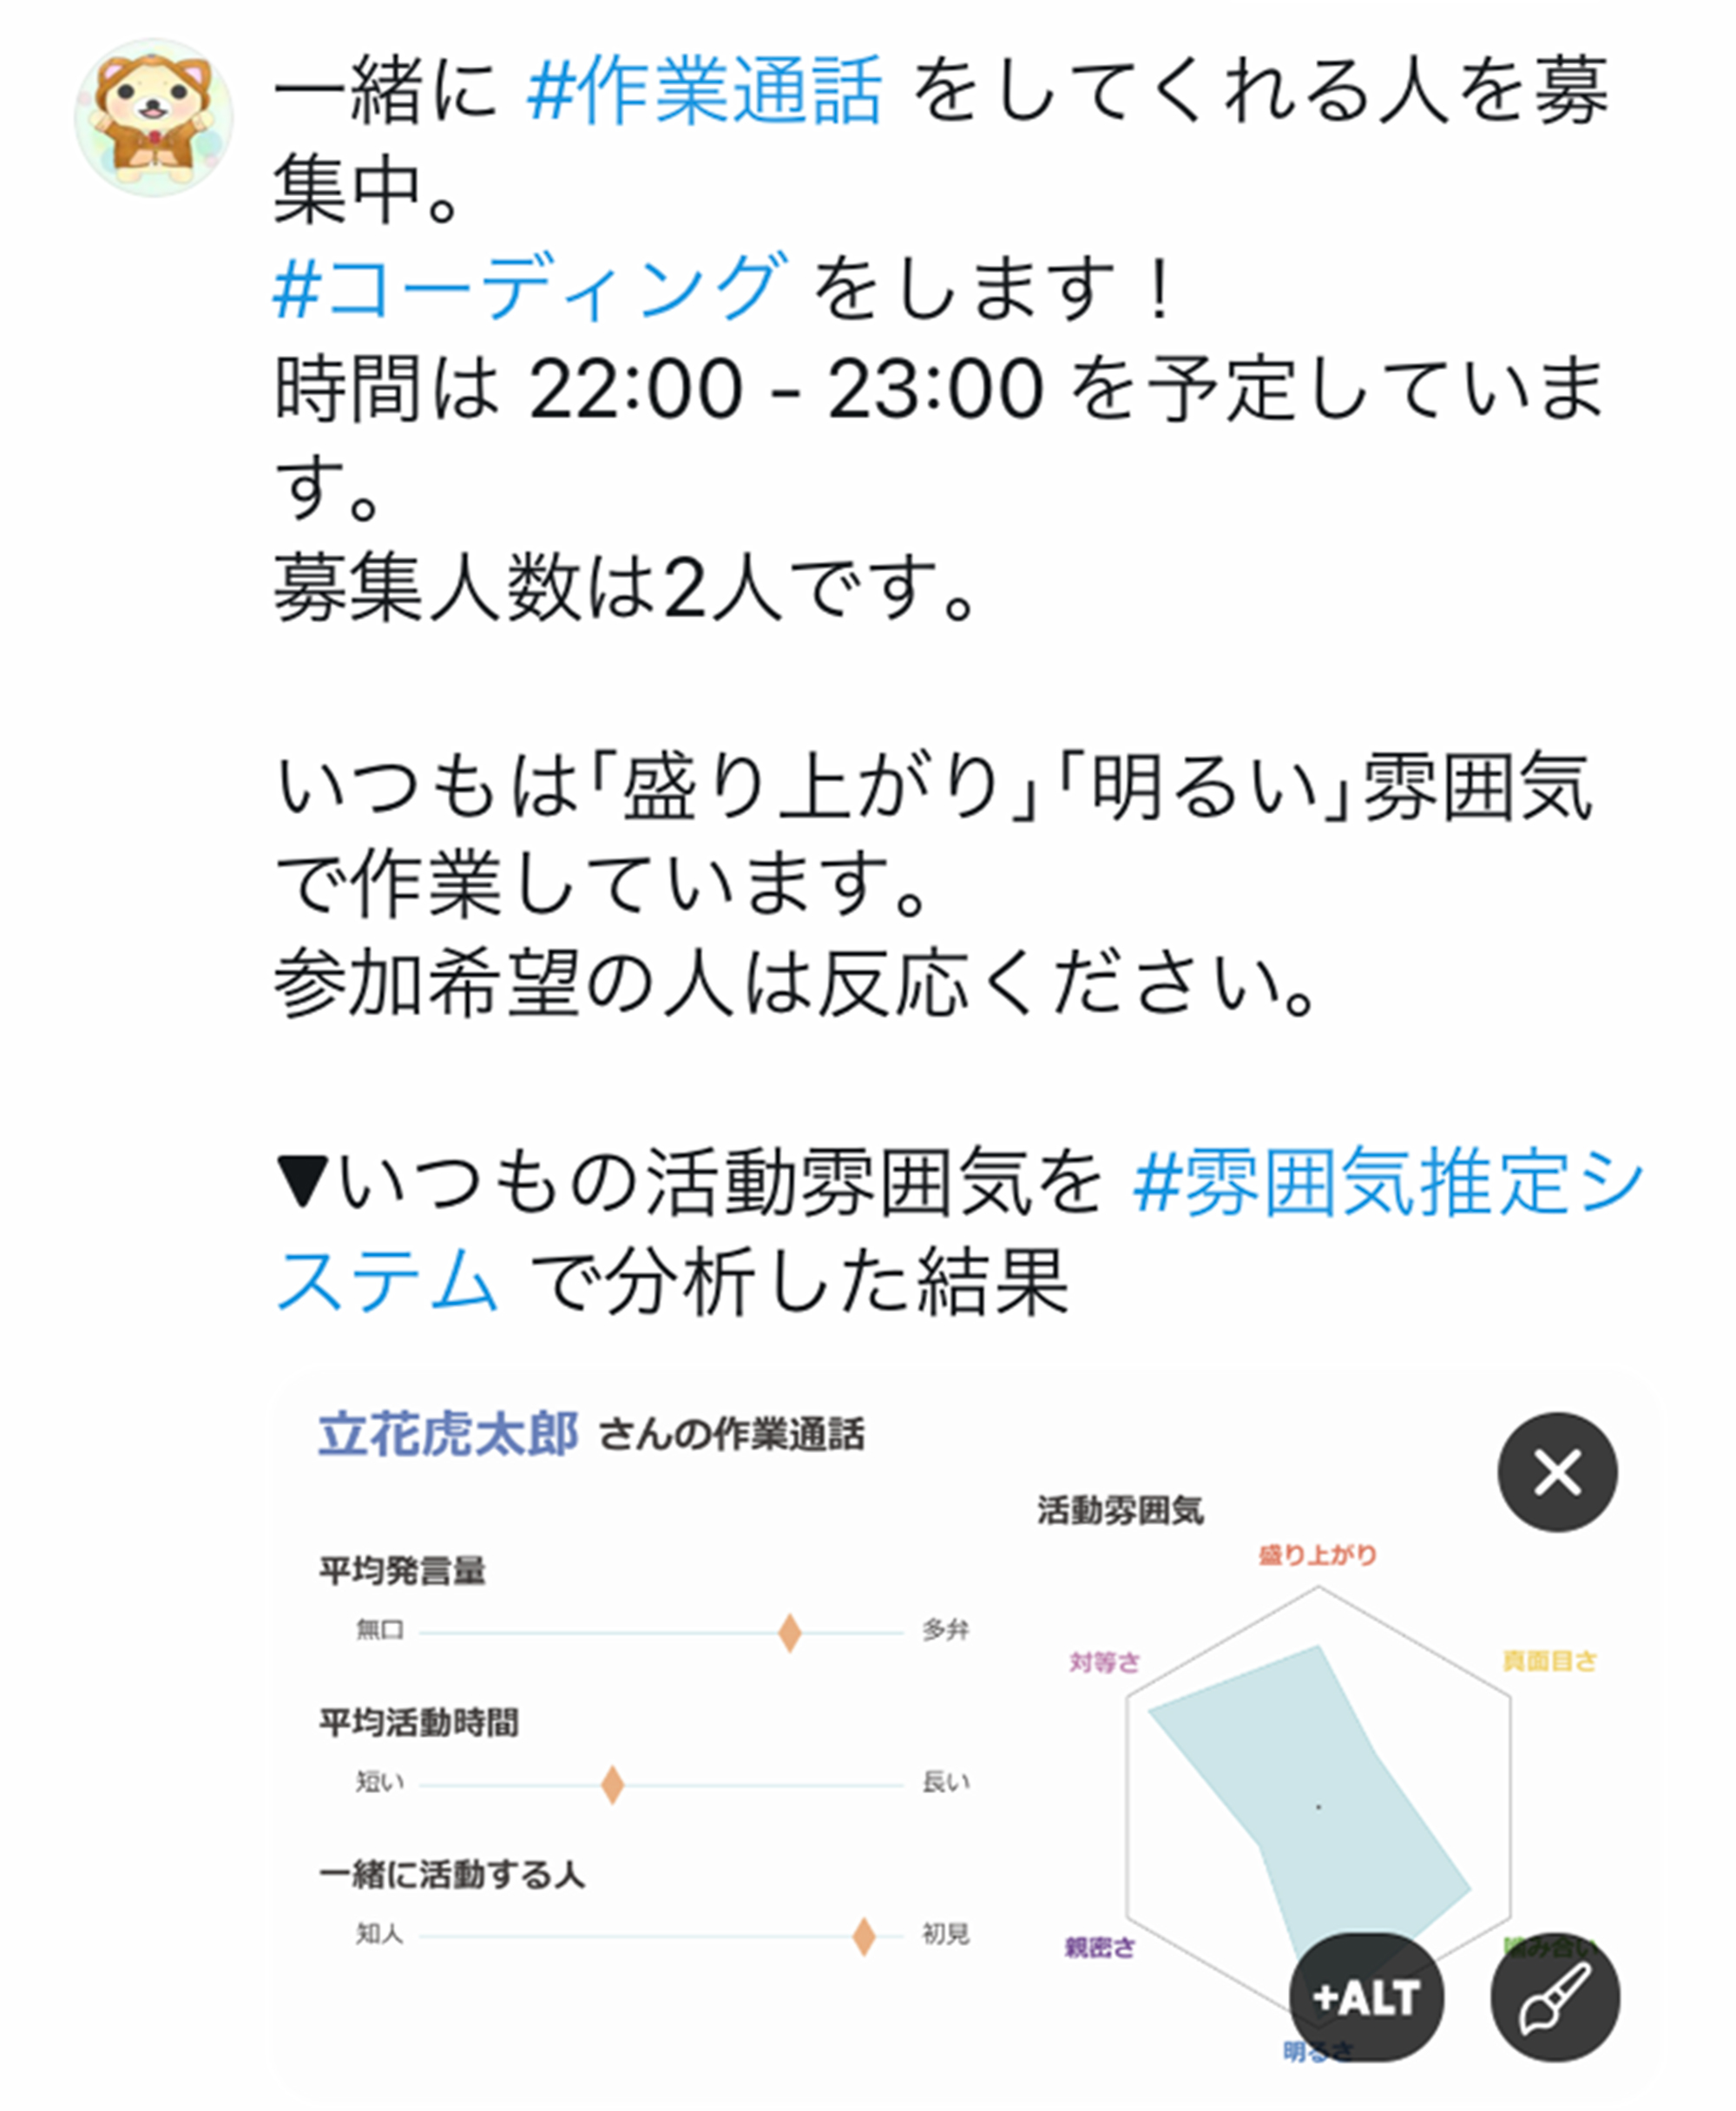
\includegraphics[width=0.7\textwidth]{figs/tweet_image.jpg}
    }
    \caption{生成する投稿のイメージ}
    \label{fig:tweet_image}
\end{figure}

本モジュールには作業嗜好の可視化機能の実装を行う(図\ref{fig:estimationgraph}).
本機能は前述した募集投稿に掲載する情報を可視化する機能である.
表示する情報は,推定された対話雰囲気の傾向値,作業時間長の平均値,雑談量の平均値,他の参加者の傾向値である.
推定された対話雰囲気の傾向値とは盛り上がっている雰囲気の対話が多いことなどをレーダーチャートにて表現した値を指し,他の参加者の傾向値とはどの程度初対面の人と積極的に作業通話を開催しているかを指す.

\begin{figure}
    \centering
    \fbox{
        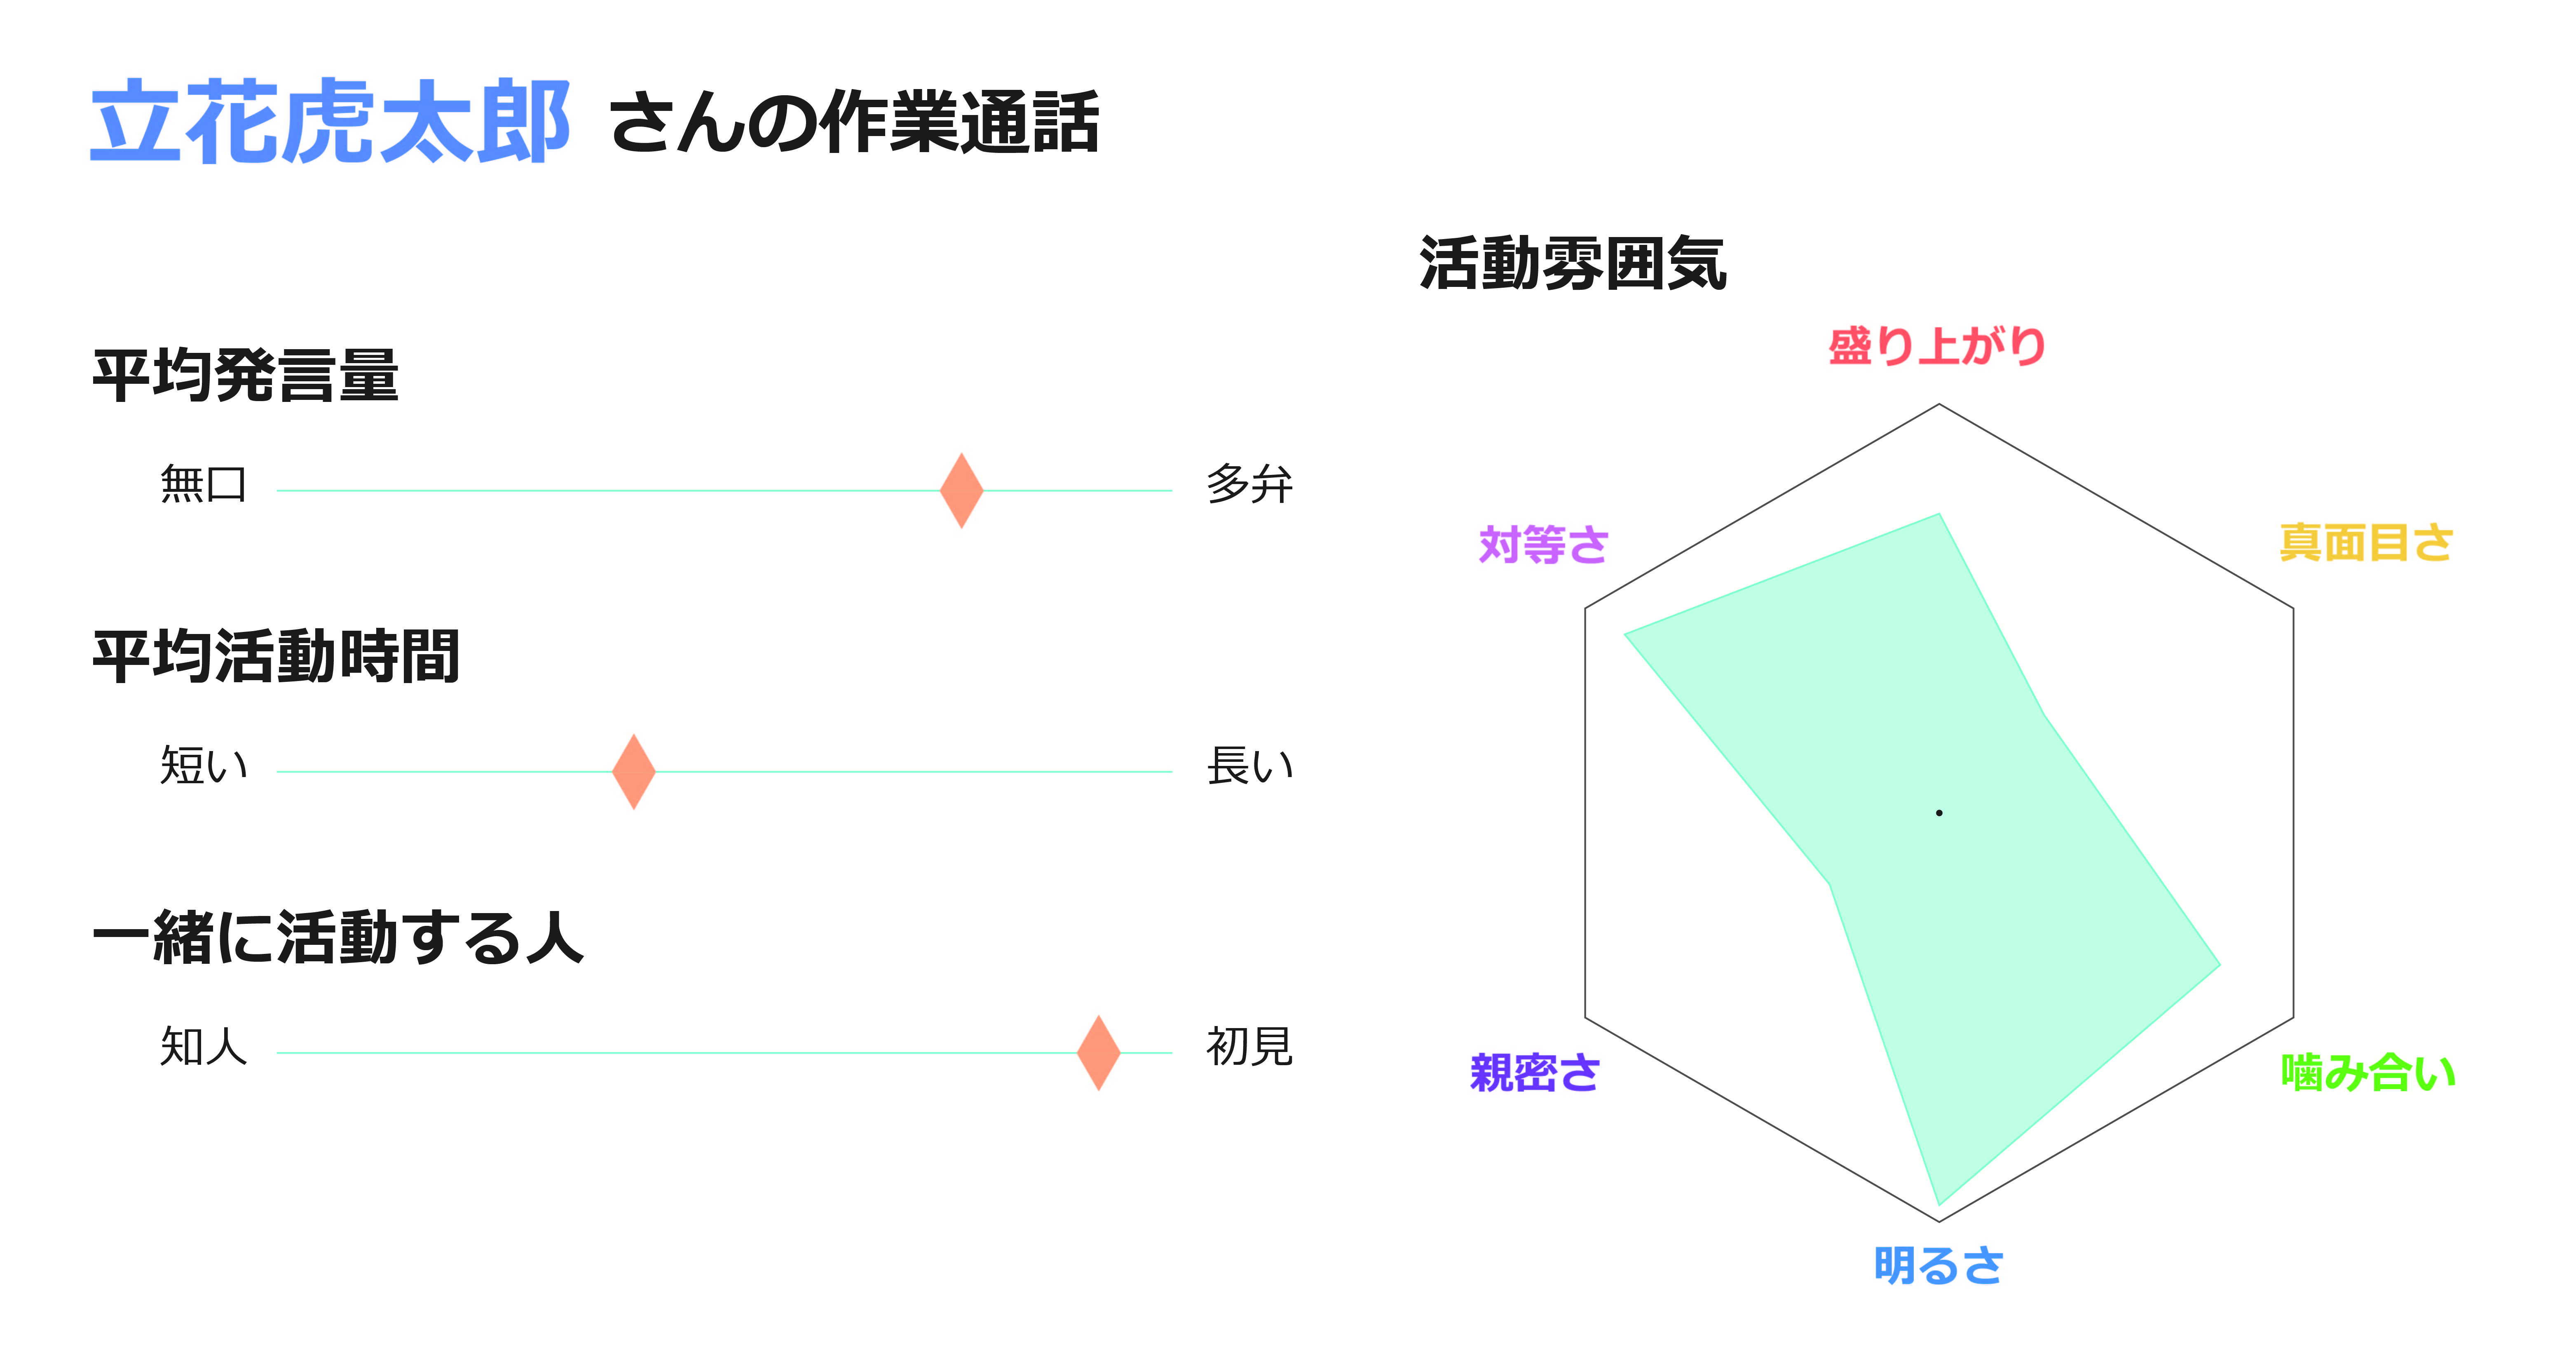
\includegraphics[width=0.7\textwidth]{figs/estimationgraph.jpg}
    }
    \caption{作業嗜好の可視化イメージ}
    \label{fig:estimationgraph}
\end{figure}

将来的には,本モジュールを用いて作業嗜好の合うユーザの推薦等無縁ユーザとの繋がり形成の機会を増加させる枠組みの構築を目指す.

\chapter{対話雰囲気推定モデル\label{sec:estimation_model}}
\thispagestyle{plain}

本章では第\ref{node:estimation_module}節で触れた対話雰囲気推定モデルの詳細について述べる.

\section{対話雰囲気モデルの構築\label{node:develop_estimation_model}}

本研究では,通話中の音声から機械学習によって対話雰囲気を推定する.
豊田らは二者対話を対象に発話時間特徴を特徴量とする機械学習を用いた対話雰囲気推定を行なっている.
豊田らの構築したモデルは「盛り上がり」「まじめさ」「噛み合い」「明るさ」「親密さ」「対等さ」の6つの雰囲気を推定対象としており,それぞれ肯定,否定の2値で分類している.
特に「盛り上がり」「まじめさ」「親密さ」の推定においては全体正答率が80%を超える高い値を示していることから,本研究でもこの手法に基づいてモデルの構築を行う.
モデルの構築手順を以下に示す.

\subsection{学習データの収集}

はじめに,学習データの収集を行う.
豊田らは音声コーパス\cite{PASD}を用いているのに対し,本研究では実際の作業通話の録音を採用する.
これは一般的な対話と作業通話中の対話は性質が異なるためである.
例えば,一般的な対話では沈黙は気まずく回避される傾向があるが,作業通話における沈黙は作業に集中していることの現れであり許容される傾向がある.
また,作業通話中の対話においては突発的な話題の変化が起こりやすく,独り言が行き交うことが多いなどの特徴がある.
このような作業通話中の対話の独特な性質が,対話雰囲気の形成に影響を与えていると十分に考えられることから,本研究では実際の作業通話の音声を学習に用いる.
学習データとして1~4名の話者からなる計6時間弱の作業通話音声の収集を行なった.
各対話の記録時間は10~120秒である.そして,各抽出データに教師ラベルを付与する.
教師ラベルは1つの抽出データに対して,推定対象の雰囲気ごとに肯定,否定のどちらかの値を与える.
本研究の推定対象雰囲気は「盛り上がり」,「真面目さ」,「親密さ」,「くつろぎ」の4つとする.
「盛り上がり」は対話の活発性や参加者の対話への積極性を指す.
「真面目さ」は対話の生産性や参加者が対話にどのくらい熱心に取り組んでいるかを指す.
「明るさ」は対話の健全さや参加者の性格を指す.
「くつろぎ」は参加への心理的安全性や対話への満足感を指す.以上の手法により,本研究では合計130対話を抽出した.

\subsection{特徴量の抽出}

各対話データから特徴量抽出のための発話集合の抽出を行う.
発話集合とは話者ごとの発話時間を記録した集合のことを指す.
また,単独発話と同時発話それぞれの発話集合を別に記録する.
以上は豊田らの手法と同様であるが,本研究ではそれに加えて全話者の発話集合を集約した全発話集合及び,全発話集合に非発話集合を加えた全集合も生成する.

生成した発話集合から特徴量の抽出を行う.
豊田らは各集合に対する統計量とその統計量を比較した値(以下,「比較量」)を算出し特徴量としている.
本研究でも統計量と比較量を特徴量とするが,具体的な算出式は異なる.
まず,それぞれの集合に対して平均値,標準偏差,最大値,要素数を算出する.
加えて,全集合以外の集合に対して占有率を算出し,全発話集合と全集合に対して合計値を算出する.
以上全てを特徴量として用いる.その後それぞれの特徴量の比較を行いそれらも特徴量とする.
これは各話者単体や全体に着目するだけでなく,各話者間や各話者と全体の比較を行うことで一部の雰囲気の推定に有効と仮説を立てたためである.
例えば,話者間に極端な発話時間・回数の差があるデータと,話者間の発話時間・回数に差があまりないデータが存在した場合,前者に比べ後者は議論が活発化しており真面目な雰囲気なことが多いのではないかと推測できる.
比較量を求める際に比較する値はそれぞれの集合の同じ統計量である.
例えば,発話時間が最も長いA話者の単独発話集合とB話者の単独発話集合を平均値で比較する場合は,A話者の単独発話集合の平均値をB話者の単独発話集合の平均値で除算することで算出する.
比較の際には話者間発話比較,話者間同時発話比較,話者内発話・非発話比較,全発話・発話比較を行う.
結果として各対話データにつき210個の特徴量が算出される.
ただし,210個というのは最大値であり実際に算出される特徴量数は話者数により異なる.
そのため,前処理として学習データ間に利用特徴量数の差があった場合は,話者数に合わせ特徴量や学習データの削除を行い新しい学習データとする.

\subsection{学習と特徴量選択}

算出された特徴量を用いて学習を行う.
本研究の学習の方法は,対象とする雰囲気や話者数が豊田らと異なるため,一部独自の手法を採用する.
本研究では,雰囲気,話者数ごとに対話雰囲気推定モデルの構築を行う.
これは各雰囲気や話者数によって有効な特徴量が異なるという仮説に基づいているためである.
本研究で学習を行う際には対象雰囲気,対象話者数,学習アルゴリズムの設定を行う.
本研究の対象雰囲気は「盛り上がり」,「真面目さ」,「明るさ」,「くつろぎ」の4つから選択する.
対象話者数は2〜4名から選択する.
学習モデルにはどの学習モデルが本研究の学習において有効であるか比較を行うため,Linear SVC,k近傍法,SVC,Naïve Bayesの4つを採用する.

また,本研究では豊田らの手法にならい,遺伝的アルゴリズム(以下,「GA」)を用いた特徴量選択を行う.
特徴量選択を行うことで精度の向上や安定化が期待できる.
具体的な手法も豊田らの手法を参考にする.
GAでは特徴量数と同じ長さのビット列からなる染色体を生成し,各特徴量の利用有無を1:有効,0:無効で表現する.
GAにおける設定の一部を表\ref{tab:ga_setting}に記載する.
表中の評価における「選択特徴量数と正答率の重み付け和による評価」は以下の式によって算出する.
式中の$W$は正答率と選択特徴量数の重み付けを表現しており,$[0, 1]$の値をとる.

\begin{table}[t]
    \caption{遺伝的アルゴリズムの設定}
    \centering
    \begin{tabular}{ll}
        \hline
        設定項目 & 範囲・候補 \\
        \hline\hline
        評価 & 正答率による評価 \\
        & 選択特徴量数と正答率の重み付け和による評価 \\
        \hline
        検証 & 交差検証の有無 \\
        \hline
        突然変異確率 & 突然変異確率 \\
        \hline
        交叉  & 一様交叉 \\
        & 二点交叉 \\
        \hline
        集団の大きさ  & 100 \\
        \hline
        エリート染色体選択数  & 20 \\
        \hline
        世代数  & 250 \\
        \hline
    \end{tabular}
    \label{tab:ga_setting}
\end{table}

\begin{equation}
    評価値 = \frac{正答数}{検証データ数} W + (1 - \frac{選択特徴量数}{全特徴量数}) (1 - W)
\end{equation}

\section{対話雰囲気モデルの評価と考察}

第\ref{node:develop_estimation_model}節で述べた手法に基づいて対話雰囲気推定モデルを構築した結果を表\ref{tab:learn_result_with_ga}に示す.
表\ref{tab:learn_result_with_ga}には各雰囲気について各話者数のモデルの学習結果の一例を掲載している.
表\ref{tab:learn_result_with_ga}に掲載している学習結果のモデルは全て特徴量選択を行ったモデルである.
表中のモデルは表\ref{tab:ga_setting}のうち評価は選択特徴量数と正答率の重み付け和による評価を採用し,突然変異率は個体突然変異率0.05,遺伝子突然変異率0.10,交叉方法には一様交叉を採用したモデルである.
評価における重み付け$W$は0.50に設定している.
また,学習アルゴリズムにはNaïve Bayesを採用している.
特徴量選択を行う前のモデルの正答率は0.7462であり,特徴量数は144個であった(「盛り上がり」を対象とした話者数3名のモデル).
同雰囲気,話者数を対象としたモデルと比較すると,特徴量選択を行うことで正答率の向上と選択特徴量数の減少が確認できる(正答率0.7956,選択特徴量数21).
加えて,雰囲気や話者数の違いによって精度に大きな差が出ていないことがわかる.
しかし,何度か学習を繰り返すと話者数の増加に伴って正答率が0.40や0.98など極端な数値になることがある.
これは学習データ数が少ないことが原因と考えられる.
例えば,検証に利用できるデータ数が2つしかない場合は正答率が0.0,0.5,1.0の3つしか取り得ない.
このように学習データが少ないことで検証を行うデータも少なくなることから極端な正答率が多く見られたと考えられる.
また,話者数の増加に伴って選択特徴量数が増加していることがわかる.
これは選択前の選択候補となる特徴量が話者数と比例して大きくなるためである.
一方で全体に対する選択割合に着目すると特に大きな差はないため,問題はないといえる.
いずれのモデルにおいても評価値に選択特徴量数を組み込むことで同様の正答率でありながら,大量の特徴量削減を行うことができることを確認した.
しかし,正答率と選択特徴量数をそれぞれどの程度重視した評価を行うかは検討の余地が残る.
二点交叉手法や,学習モデルとしてLinear SVC,k近傍法,SVCを用いたモデルなどを構築したが表中のモデルとの大きな差は確認できなかった.

\begin{table}[t]
    \caption{特徴量選択を用いたモデルの学習結果}
    \centering
    \begin{tabular}{|c|c|r|r|}
        \hline
        雰囲気 & 話者数 & 正答率 & 選択特徴量数 \\
        \hline\hline
        \multirow{3}{*}{盛り上がり} & 2 & 0.8000 & 10 \\
        & 3 & 0.7956 & 21 \\
        & 4 & 0.8600 & 45 \\ \hline
        \multirow{3}{*}{真面目さ} & 2 & 0.7752 & 16 \\
        & 3 & 0.7694 & 30 \\
        & 4 & 0.8000 & 38 \\ \hline
        \multirow{3}{*}{明るさ} & 2 & 0.8305 & 12 \\
        & 3 & 0.8639 & 33 \\
        & 4 & 0.7000 & 40 \\ \hline
        \multirow{3}{*}{くつろぎ} & 2 & 0.7905 & 13 \\
        & 3 & 0.8167 & 25 \\
        & 4 & 0.9000 & 40 \\ \hline
    \end{tabular}
    \label{tab:learn_result_with_ga}
\end{table}

本研究の対話雰囲気推定モデルは対話単位のデータを入力値としている.
そのため,実際の作業通話にDiscord Botを用いて自動で雰囲気推定を行う場合は,適切なタイミングで話題の切り替わりを判断し,一つのデータとして評価する必要がある.
しかし,本研究で収集する音声データは発話状態時間特徴のみであるため,言語情報を用いた切り替わり判断を行うことができない.
現在は,1 〜 2秒の無音時間を検知した際にデータを切り分けることで,話題の切り替わりを判断する手法を検討している. 


\chapter{評価実験\label{sec:evaluation_experiment}}
\thispagestyle{plain}

本章では,本研究において構築した対話雰囲気推定モデル及び,それを用いたDiscord Botの評価実験について述べる.

\section{概要}

本研究では対話雰囲気推定モデル及び,Discord Botの評価実験を行う.
雰囲気の一致率やシステムの利便性など主観に基づいた評価を行うため,どちらの評価実験においてもアンケートを用いる.

対話雰囲気推定モデルの評価実験では,モデルの妥当性の評価を目的に,被験者が感じる対話雰囲気とモデルの推定結果がどの程度一致しているかを調査する.
被験者は一度でも作業通話に参加したことがある人とする.
これは作業通話の雰囲気を過去の開催記憶と照らし合わせながら評価をしてもらうことでより説得力のある評価とするためである.
手順はまず本研究の主旨や用語の説明をし,いくつかの対話を聞いてもらいアンケート調査を行う.
調査項目としては「対話を聞いてどのような雰囲気を感じたか」や「対話雰囲気推定モデルの推定結果についてどのように感じたか」などを検討している.
それらの回答をもとに,対話雰囲気推定モデルの推定結果の妥当性を評価する.

Discord Botの評価実験では,Botの利便性の評価を目的に調査を行う.
被験者は対話雰囲気推定モデルの評価実験同様,日常的に作業通話を開催している人とする.
手順はまずBotの利用方法を説明したのちに,Botを交えた短時間の作業通話を行い,出力結果や使用感についてのアンケート実施する.
調査項目としては「Bot操作や表示方法で不明点や不便な点がなかったか」や「雰囲気の修正をしたいと感じたか」などを検討している.
それらの回答をもとに,Discord Botの利便性を評価する.

\chapter{結論\label{sec:conclusion}}
\thispagestyle{plain}

本論文では対話雰囲気推定を用いた作業通話の進め方の可視化手法の提案及び構築と,それを用いた参加者募集システムの提案を行なった.
今後は6章で述べた課題の解決と7章で述べた評価実験を行う.
その後はより多くの学習データを用いた学習を行うことで,より精度が高く安定した対話雰囲気推定モデルの構築を行うことを検討している.
また,モデルの構築後は3章で述べた作業通話マッチング支援システムの構築及び検証を行うことを検討している.
その際にはより多くの人が利用しやすいUIやUXも踏まえてシステムを検討していく.

将来的には作業通話だけでなくオンラインゲームの通話を始めとした複数人による通話全般の活動雰囲気の推定等に応用できる対話雰囲気推定モデルやシステムの構築を期待している.


% TODO: 謝辞
\pagestyle{plain}
\chapter*{謝辞}

本研究を進めるにあたり,お忙しい中ご指導いただいた奥野拓教授に深くお礼申し上げます.
また,様々な助言をくださった研究室の後輩方や同期の学生にも深くお礼申し上げます.


% TODO: 発表等実績
\chapter*{発表・採録実績}

% TODO: 発表・採録実績(確定分も含む)を以下の例のように記入

\subsection*{発表等}
\begin{enumerate}
\renewcommand{\labelenumi}{[\arabic{enumi}]}
    \item 立花虎太郎・奥野拓, 雰囲気推定を用いた作業通話マッチング支援システムの提案, 第118回グループウェアとネットワークサービス・第36回コンシューマ・デバイス&システム・第33回デジタルコンテンツクリエーション合同研究発表会, 2023-01-24, 発表予定.
\end{enumerate}



% TODO: 参考文献
% TODO: 参考文献を以下のように記入.

\begin{thebibliography}{99}
\bibitem{Discord}
``Discord'': https://discord.com/, (参照 2023-01-12).
\bibitem{Zajonc}
Zajonc, R, B.: Social facilitation, Science, Vol.149, pp.269-274, 1965.
\bibitem{Matsumoto}
松本芳之:観察者効果に関するフィード研究:技能水準,課題難度,遂行状況の関係について,実験社会心理学研究,Vol.26,No.2,pp.115-123,1987.
\bibitem{Miyamoto}
宮本正一:観察者の存在による選択反応時間の抑制,心理学研究,Vol.58,No.4,pp.240-246,1987.
\bibitem{Twitter}
``Twitter'': https://twitter.com/, (参照 2023-01-12).
\bibitem{Harada}
原田悦子:人の視点から見た人工物研究(認知科学モノグラフ6),共立出版,1997.
\bibitem{Kimura}
木村泰之,都築誉史:集団意思決定とコミュニケーション・モードコンピュー夕・コミュニケーション条件と対面コミュニケーション条件の差異に関する実験社会心理学的検討,実験社会心理学研究,Vol.38,pp.183-192,1998.
\bibitem{Nishimura}
西村洋一:対人不安、インターネット利用、およびインターネットにおける対人関係,社会心理学研究,Vol.19,pp.124-134,2003.
\bibitem{Tsuzuki}
都築誉史,木村泰之:大学生におけるメディア・コミュニケーションの心理的特性に関する分析一対面、携帯電話、携帯メール、電子メール条件の比較,立教大学応用社会学研究,Vol.42,pp.15-24,2000.
\bibitem{Tokuhisa}
徳久良子,寺嶌立太:雑談における発話のやりとりと盛り上がりの関連,人工知能学会論文誌,Vol.21,No.2A,pp.133-142,2006.
\bibitem{Ito}
伊藤秀樹,重野真也,西本卓也,荒木雅弘,新美康永:対話における雰囲気の分析,情報処理学会研究報告 SLP,音声情報処理,Vol.2002,No.10,pp.103-108,2002.
\bibitem{Toyota}
豊田薫,宮越喜浩,山西良典,加藤昇平:発話状態時間長に着目した対話雰囲気推定,人工知能学会論文誌,Vol.27,No.2SP-B,pp.16-21,2012.
\bibitem{Kitamura}
北村太一,小川祐樹,諏訪博彦,太田敏澄:コミュニケーションに着目したTwitterフォローユーザ推薦,人工知能学会全国大会論文集,Vol.26,pp.1-4,2012.
\bibitem{Tamura}
田村政人,小林亜樹:Twitterにおける会話しやすいユーザの推薦手法,情報処理学会第75回全国大会講演論文集,Vol.2013,No.1,pp.605-607,2013.
\bibitem{Kume}
久米雄介,打矢隆弘,内匠逸:興味領域を考慮したTwitterユーザ推薦手法の提案と評価,情報処理学会研報告 SIG,Vol.2015-ICS-179,No.1,pp.1-8,2015.
\bibitem{Hikawa}
樋川一幸:適切な距離の学生に依頼可能なBotを利用した実験協力者募集手法の研究,明治大学大学院先端数理科学研究科修士(工学),2020. 
\bibitem{LINE}
``LINE'': https://line.me/ja/, (参照 2023-01-12).
\bibitem{PASD}
NII音声資源コンソーシアム:対話音声コーパス(PASD),1996.
\end{thebibliography}


% 図表一覧等自動生成
\listoffigures
\thispagestyle{plain}
\listoftables
\thispagestyle{plain}


\end{document}
